


\chapter{Przeprowadzone badania}
\section{Projekt klasyfikatora}

\section{Opis platformy i w jaki sposób zrealizowano badania}

\subsection{Język python}
Wszystkie badania i testy zostały napisane z wykorzystaniem języka python. Jest to język programowania interpretowany, wysokiego poziomu z dużą ilością dostępnych bibliotek. Python\cite{python} posiada dynamiczne zarządzanie typami oraz automatyczne zarządzanie pamięcią. Wspiera kilka paradygmatów programowania, takich ja: obiektowy, imperatywny, funkcyjny i proceduralny. Został zaprojektowany z myślą o czytelności kodu oraz składnią pozwalającą napisać program z mniejszą ilością kodu niż w językach C++ lub Java. Implementacje języka python dostępna jest na wiele systemów operacyjnych. Często wykorzystywany jest jako język skryptowy. Python jest projektem typu Open Source. \par
W pracy wykorzystano język python w wersji 2.7.11. Język ten wybrano ze względu na łatwość pisania w nim kodu, szybką możliwość nauki oraz na szeroki wachlarz dostępnych bibliotek. Ważnym argumentem w wyborze były gotowe biblioteki z klasyfikatorami oraz do pracy z klasyfikacją danych. Dostępność bibliotek do wizualizacji dla tego języka, pozwoliła na przedstawienie wyników testów w formie graficznej. Napisane testy, można w łatwy sposób rozbudować, zmodyfikować lub dodać nowe elementy.    

\subsection{Biblioteka scikit-learn}
Scikit-learn\cite{scikit} to proste i wydajne narzędzie do analizy i eksploracji danych. Jest to biblioteka uczenia maszynowego dla języka python. Rozpowszechnianie oparta jest na licencji BSD. W Scikt-learn zaimplementowane są (lub napisany jest kod obsługujący) różne algorytmy klasyfikacji, regresji, analizy skupień takie jak: maszyna wektorów nośnych, algorytmy najbliższego sąsiada, naiwny Bayes, drzewa decyzyjne, sieć neuronowa, zespoły klasyfikatorów. Z wykorzystaniem tej biblioteki można przygotować oraz przetworzyć odpowiednio dane. Możliwe jest także, ocenianie i wizualizacja wyników. \par
W testach użyto biblioteki scikit-learn w wersji 0.18.1. Wykorzystano z niej algorytmy klasyfikacji oraz wstępnego przetwarzania danych.
\subsection{Biblioteka imbalanced-learn}
Biblioteka imbalanced-learn\cite{imlearn} zawiera zestaw narzędzi do wstępnego przetwarzania danych niezrównoważonych. Posiada ona zaimplementowane różne metody under- oraz over-sampling do równoważenia zbiorów danych. W pracy wykorzystano te metody z biblioteki w wersji 0.2.1. 
\subsection{Pozostałe użyte biblioteki}
\subsubsection{Mlxtend}
Mlxtend (machine learning extensions)\cite{mlxtend} jest to biblioteka zawierająca różne narzędzia do pracy z danymi. W badaniach wykorzystano z niej algorytm Stacking.
\subsubsection{Numpy}
Numpy to pakiet umożliwiający obliczenia naukowe. Szczególnym elementem jest możliwość wykonywania obliczeń na tablicach N-wymiarowych. 
\subsubsection{Maptolib}
Maptolib to biblioteka pythona, która tworzy różnego rodzaju wykresy 2D oraz interaktywne na różnych platformach.
\subsubsection{Texttable}
Texttable to prosty moduł napisany w języku python, służący do produkcji prostych tabel ASCII. Został wykorzystany do prezentacji wyników w konsoli.
\subsubsection{Pylatex}
Pylatex to biblioteka pythona, służąca do tworzenia i kompilacji plików LaTeX. W pracy została wykorzystana do zapisu wyników w badań w plikach .tex oraz .pdf.
\subsection{opisac co zaimplementowane?}
\todo{ze wlasna krosswalidacja, ze wlasne miary, klasyfikator. itd}

\todo{inline} napisac o roznych F i o tym jak wyniki wyglada, pokazać test

\section{Opis danych użytych w badaniach}
Do przeprowadzenia badań użyto 26 różnych prawdziwych zbiorów danych (tabela \ref{danebadania}) pochodzących z repozytorium serwisu "The UCI Machine Learning Repository" \cite{uci}. Dane wybrano ze względu na różnorodność typów danych, ilości rekordów, atrybutów oraz zróżnicowanie rozkładu klas. Większość z danych była używana w publikacjach podobnych tematycznie\cite{hyper}\cite{StefImbalanced}. \par
Wszystkie dane zostały zapisane w skrypcie, w folderze $praca/data/files$, a opis szczegółowy danych znajduje się w folderze $praca/data/files/data\_descrytpion$. Do importu danych służą funkcje z pliku $praca/data/import\_data.py$. Do ogólnego importu danych z pliku, służy funkcja $importfile$, zaś wczytywanie danych użytych w projekcie odbywa się poprzez funkcje zaczynające się od $load\_$. Import danych z pliku odbywa się z wykorzystaniem funkcji z pakietu $numpy$ $genfromtext$ oraz $load\_txt$. Atrybuty posiadające dane kategoryczne zapisane w postaci łańcuchów znaków zostały zamienione na dane numeryczne. Cechy nominalne zostały zakodowane metodą $one hot encoding$. Dla danych zawierających więcej niż dwie klasy, klasa z najmniejszą liczebnością została wybrana jako klasa mniejszościowa, pozostałe klasy utworzyły klasę większościową. We wszystkich zbiorach danych, kategorie reprezentowane są w systemie binarnym. 5 zbiorów danych posiadało brakujące wartości. Zostały one zastąpione wartościami środkowymi zbioru (medianą).
\begin{table}[H]
	\begin{center}
		\resizebox{\textwidth}{!}{%
			\begin{tabular}{|c|c|c|c|c|c|}%
				\hline%
				Nazwa danych&L. el.&Atrybuty&Rozklad klas&\% kl. mn.&IR\\%
				\hline%
				abalone0\_4&4177&8&4103/74&1.77&55.45\\%
				abalone041629&4177&8&3842/335&8.02&11.47\\%
				abalone16\_29&4177&8&3916/261&6.25&15.0\\%
				balance\_scale&625&4&576/49&7.84&11.76\\%
				breast\_cancer&286&9&201/85&29.72&2.36\\%
				bupa&341&6&200/141&41.35&1.42\\%
				car&1728&6&1663/65&3.76&25.58\\%
				cmc&1473&9&1140/333&22.61&3.42\\%
				ecoli&336&7&301/35&10.42&8.6\\%
				german&1000&24&700/300&30.0&2.33\\%
				glass&214&9&197/17&7.94&11.59\\%
				haberman&306&3&225/81&26.47&2.78\\%
				heart\_cleveland&303&13&268/35&11.55&7.66\\%
				hepatitis&155&19&123/32&20.65&3.84\\%
				horse\_colic&368&22&232/136&36.96&1.71\\%
				ionosphere&351&34&225/126&35.9&1.79\\%
				new\_thyroid&215&5&185/30&13.95&6.17\\%
				postoperative&90&8&66/24&26.67&2.75\\%
				seeds&210&7&140/70&33.33&2.0\\%
				solar\_flare&1066&10&1023/43&4.03&23.79\\%
				transfusion&748&4&569/179&23.93&3.18\\%
				vehicle&846&18&647/199&23.52&3.25\\%
				vertebal&310&6&210/100&32.26&2.1\\%
				yeastME1&1484&8&1440/44&2.96&32.73\\%
				yeastME2&1484&8&1433/51&3.44&28.1\\%
				yeastME3&1484&8&1321/163&10.98&8.1\\%
				\hline%
			\end{tabular}}
			\caption{Dane użyte w badaniach wraz z charakterystyką.}
			\label{danebadania}
		\end{center}
	\end{table}
\todo{opisac foldy w zaleznosci od ilosci danych}
\section{Sposób mierzenia w sprawdzianie krzyżowym}
\section{Ocena klasyfikatora w sprawdzianie krzyżowym k-krotnym.}
W większości publikacji naukowych dotyczących klasyfikacji, ocena klasyfikatora mierzona jest z wykorzystaniem sprawdzianu krzyżowego (zwykle k=10) oraz przedstawionych wcześniej miar. Jednakże, w tych publikacjach nie został opisany sposób obliczania współczynników w czasie sprawdzianu krzyżowego. Wykorzystanie różnych sposobów, prowadzi do różnych wyników. Niektóre metody są mniej lub bardziej obciążone błędem. Różnice w wynikach, wynikające z przyjętej metody obliczeniowej, są szczególnie widoczne w sprawdzianie krzyżowym z losowym rozkładem danych oraz w klasyfikacji danych niezrównoważonych. Są dwie główne możliwości obliczania współczynników:
\begin{itemize}
	\item obliczanie wartości współczynników dla każdej k-iteracji (klasyfikatora), a następnie obliczenie średniej z tych iteracji
	\item stworzenie jednej wspólnej macierzy pomyłek dla każdej k-iteracji, a następnie obliczenie wskaźników.
\end{itemize}
W przypadku drugiego sposobu, poszczególne elementy macierzy pomyłek będą wynosić odpowiednio:
\[TP := \sum_{i=1}^{k} TP^{(i)}\]
\[FP := \sum_{i=1}^{k} FP^{(i)}\]
\[TN := \sum_{i=1}^{k} TN^{(i)}\]
\[FN := \sum_{i=1}^{k} FN^{(i)}\]
\subsection{Test sposobów oceny klasyfikatora}
W celu wyboru najlepszego sposobu oceny klasyfikatora, z najmniejszym błędem oraz wariancją wykonano pięć porównujących testów dla różnych metod obliczania miar. Wszystkie testy miały takie same założenia oraz sposób wykonania. Testy wykonano na wygenerowanych losowo danych dla różnej ilości przykładów pozytywnych (od 1\% do 10\%). Jakość klasyfikacji była oceniana dla równomiernego sprawdzianu krzyżowego oraz dla losowego. Symulacje odbyły się one w następujący sposób:

\begin{enumerate}
	\item Wygeneruj zbiór 1500 losowych próbek z 2 atrybutami, 2 klasami o rozkładzie 4:1
	\item Wykonaj niezrównoważenie zbioru z ratio 0.1
	\item Wybierz m=[1..10]*10 przykładów klasy mniejszościowej oraz 1000-m przykładów klasy dominującej
	\begin{enumerate}
		\item  Wykonaj N iteracji:
		\begin{enumerate}
			\item Wymieszaj dane
			\item Wykonaj sprawdzian krzyżowy k-krotny, k=10
			\item Oblicz współczynniki dla obu metod
		\end{enumerate}
		\item Oblicz odchylenie standardowe oraz średnie wartości współczynników
	\end{enumerate}
	\item Przedstaw wyniki odchylenia standardowego oraz średnie wartości współczynników dla różnego rozkładu klas.
\end{enumerate}
Wykonanie testu N-krotnie (najlepiej n>100000) pozwala na obliczenie "prawdziwych" wartości miar oceny klasyfikacji. Powtórzenie sprawdzianu krzyżowego wielokrotnie pozwala na ocenę błędu oraz wariancji miar dla każdej metodyki. Przeprowadzenie testu dla danych zawierających tylko 1\% obserwacji klasy mniejszościowej (przypadek ekstremalny, w zbiorze danych znajduje się wtedy tylko 10 takich przykładów) oznacza, że w niektórych iteracjach sprawdzianu krzyżowego nie będzie przykładów poprawnie sklasyfikowanych z tej klasy. Brak dobrze sklasyfikowanych przykładów klasy mniejszościowej może mieć także miejsce w losowym sprawdzianie krzyżowym. Wynika to z braku równomiernego rozkładu obu klas. 
\subsubsection{Dokładność oraz błąd klasyfikatora}
Dokładność klasyfikacji oraz błąd klasyfikatora, korzystając z metody pierwszej, będzie wynosić:
\[accuracy_{avg} := \frac{1}{k} \sum_{i=1}^{k} accuracy^{(i)}\]
a błąd klasyfikatora:
\[error\ rate_{avg} = 1 - accuracy_{avg}\]
Obliczając drugim sposobem, korzysta się z podstawowego wzoru z wykorzystaniem wspólnej macierzy pomyłek. \par
W przypadku dokładności oraz błędu klasyfikatora, niezależnie od przyjętej metodyki otrzymane wartości będą takie same, nieobciążone błędem.
\subsubsection{Czułość, specyficzność, FPR oraz precyzja}
Czułość, specyficzność, FPR oraz precyzja w metodzie pierwszej obliczą się wg. wzorów:
\[Sensitivity_{avg},\ Recall_{avg},\ TPR_{avg} := \sum_{i=1}^{k} TPR_{avg}^{(i)}\]
\[Specificity_{avg},\ TNR_{avg} := \sum_{i=1}^{k} TNR_{avg}^{(i)}\]
\[FPR_{avg} := \sum_{i=1}^{k} FPR_{avg}^{(i)}\]
\[Precision_{avg} := \sum_{i=1}^{k} Precision_{avg}^{(i)}\]
W drugim sposobie korzysta się z wspólnej macierzy pomyłek oraz z podstawowych wzorów. \par
Testy wyżej wymienionych współczynników, zostały przeprowadzone z wykorzystaniem skryptu $test\_wsk.py$. Zauważono, że w przypadku równomiernego sprawdzianu krzyżowego, różnica w wynikach jest bardzo mała, poniżej 0.5\%. Obie metody obarczone sa małym błędem i wariancją. Natomiast w przypadku sprawdzianu krzyżowego z rozkładem losowym, metoda druga okazała się lepsza. Obliczona czułość oraz precyzja sposobem drugim, uzyskały wyniki z mniejszym błędem, bliższe wartości "prawdziwej". Natomiast specyficzność w obu metodach wyszła taka sama, ze względu na dużą ilość przykładów z tej klasy. Zostało sprawdzone, że w momencie odwrócenia liczebności klas, specyficzność posiada taką samą charakterystykę jak czułość. Różnice w wynikach obu sposobów, zmniejszają się wraz ze wzrostem przykładów klasy większościowej. Zazwyczaj przy 10\% zawartości danych klasy zdominowanej w zbiorze, wyniki są takie same.
\begin{figure}[H]
	\centering
	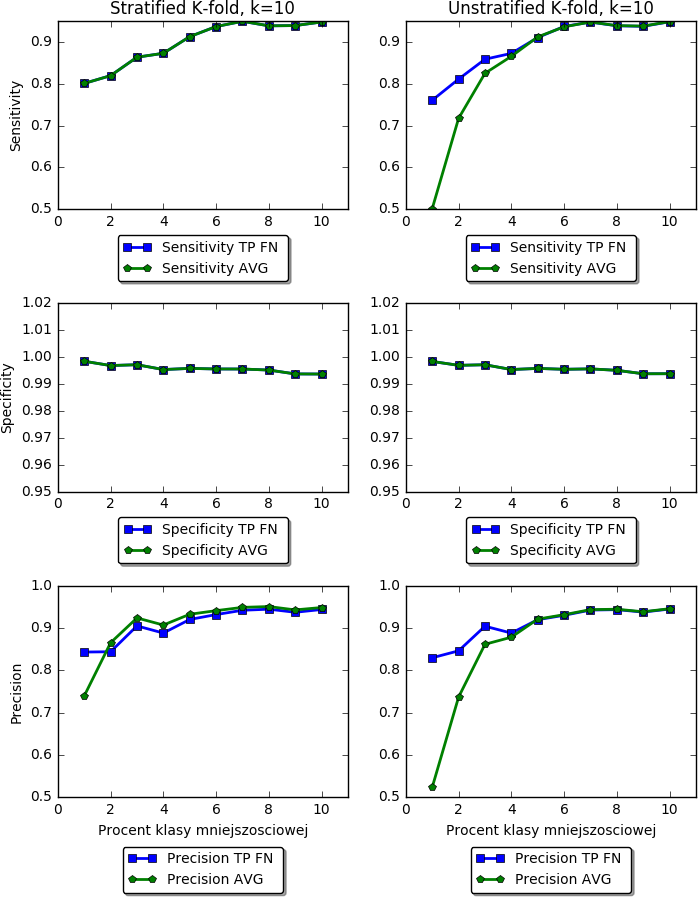
\includegraphics[width=\textwidth]{./images/wsk.png}
	\caption{Wykresy czułości, specyficzności oraz precyzji w zależności od wielkości klasy mniejszościowej dla równomiernego oraz losowego sprawdzianu krzyżowego (k=10).}
	\label{fig:wskazniki}
\end{figure}

\begin{figure}[H]
	\centering
	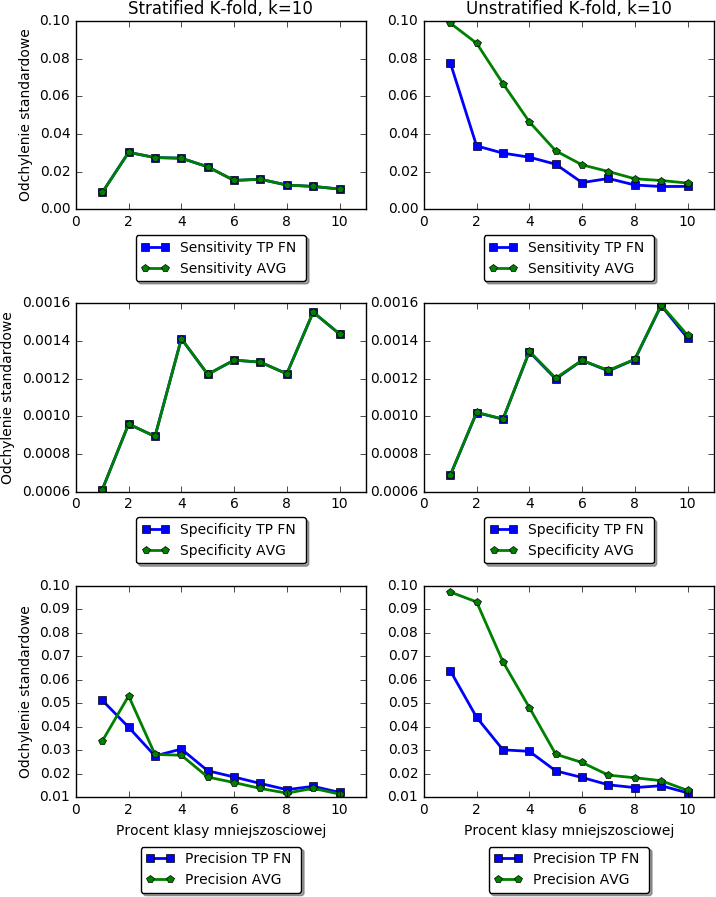
\includegraphics[width=\textwidth]{./images/stdwsk.png}
	\caption{Odchylenie standardowe miar czułości, specyficzności oraz precyzji w zależności od wielkości klasy mniejszościowej dla równomiernego oraz losowego sprawdzianu krzyżowego (k=10).}
	\label{fig:wskaznikistd}
\end{figure}
\todo{wstawic wykres i opisac}
\subsubsection{Miara $F_1$}
W niniejszej pracy oraz w dużej ilości publikacjach miara F-measure obliczana jest dla $\beta=1$, dlatego testy przeprowadzono tylko dla tej wartości. Miarę F, można obliczyć na trzy różne sposoby. Pierwszy polega na obliczeniu F dla każdego k klasyfikatora, a następnie uśrednienie wyników:
\[F_{avg} := \frac{1}{k} \sum_{i=1}^{k} F_1^{(i)}\]
Drugi sposób, to obliczenie średniej czułości i precyzji, a następnie miary F z podstawowego wzoru:
\[Pre_{avg} := \frac{1}{k} \sum_{i=1}^{k} Pre^{(i)}\]
\[Re_{avg} := \frac{1}{k} \sum_{i=1}^{k} Re^{(i)}\]
\[F_{pre, re} = 2 * \frac{Pre_{avg}*Re_{avg}}{Pre_{avg}+Re_{avg}} \]
Ostatnio sposób, to obliczenie współczynnika F ze wspólnej, końcowej macierzy pomyłek:
\[F_{tp, fp, fn} = \frac{2*TP}{2*TP+FP+FN} \]
Do powyższych wzorów można dodać jeszcze sposób odrzucający oceny klasyfikatorów, dla których precyzja lub czułość są niezdefiniowane. Ta metoda została odrzucona ze względu na zawyżanie końcowej oceny. \par 
Skrypt testujący powyższe trzy sposoby znajduje się w pliku $test\_f1.py$. Analizując otrzymane wyniki (wykres \ref{fig:wykresf1}), zauważono, że najbardziej powtarzalne wyniki otrzymano korzystając z wzoru $F_{tp, fp, fn}$. W przypadku obu sprawdzianów krzyżowych, metoda ta generowała najmniejszy błąd. Zauważono, że niezależnie od ilości danych niezrównoważonych, otrzymane wyniki tą metodą różniły się nieznacznie, w przeciwieństwie do pozostałych sposobów. Podobnie jak w przypadku poprzednich miar, wraz ze wzrostem ilości danych niezrównoważonych, uzyskiwane wyniki były prawie takie same, niezależnie od sposobu obliczania.
\begin{figure}[H]
	\centering
	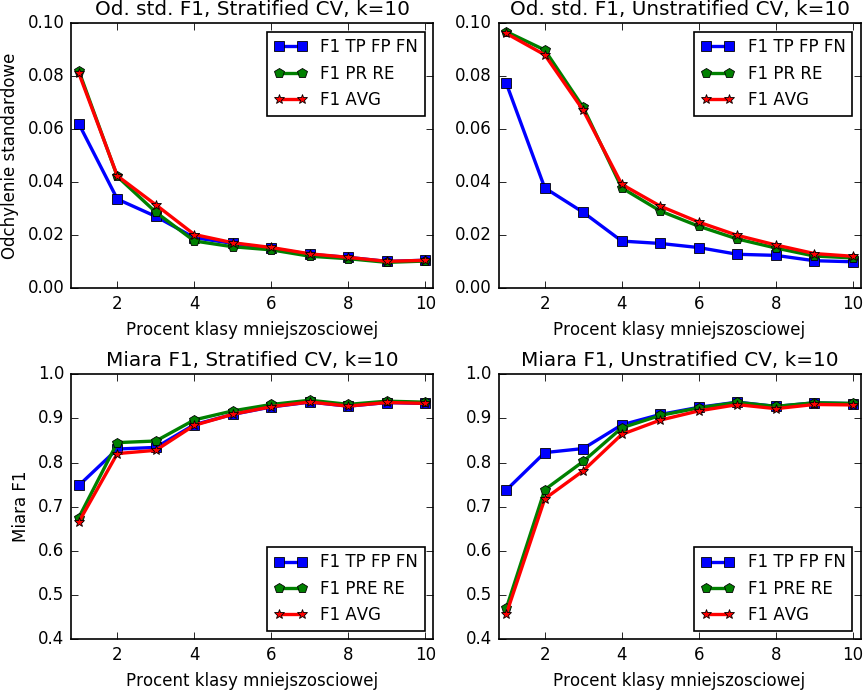
\includegraphics[width=\textwidth]{./images/miara-F1.png}
	\caption{Wykres odchylenia standardowego miar F1 oraz średniej miar F1 w zależności od wielkości klasy mniejszościowej dla równomiernego oraz losowego sprawdzianu krzyżowego (k=10).}
	\label{fig:wykresf1}
\end{figure}
\subsubsection{Miara G-mean}
Miara G-mean może zostać obliczona również na trzy różne sposoby. Pierwszy z nich to średnia z wszystkich klasyfikatorów:
\[G-mean_{avg} := \frac{1}{k} \sum_{i=1}^{k} G-mean^{(i)} \]
W drugim sposobie należy najpierw obliczyć średnią wartość czułości oraz specyficzności, a końcowy wynik G-mean oblicza się z głównego wzoru:
\[G-mean_{Se, Sp} = \sqrt{Sensitivity_{avg}*Specificity_{avg}} \]
W ostatniej metodzie obliczania G-mean, za czułość oraz specyficzność, wstawia się właściwie wzory, a wartość oblicza się na podstawie zsumowanej macierzy pomyłek.
\[G-mean_{tp, fp, fn} = \sqrt{\frac{TP}{TP + FN}*\frac{TN}{TN + FP}} \]
Skrypt testujący powyższe wzory znajduje się w pliku $test\_g\_mean.py$. Analizując wyniki (wykres \ref{fig:wykresgmean}) równomiernego sprawdzianu krzyżowego, zaobserwowano, że  wyniki $G-mean_{tp, fp, fn}$ oraz $G-mean_{Se, Sp}$ pokrywają się. Natomiast w zwykłym sprawdzianie krzyżowym, pomiarem najmniej obarczonym błędem był $G-mean_{tp, fp, fn}$. Z wykorzystaniem tego wzoru, dla różnej zawartości klasy mniejszościowej w zbiorze danych otrzymano wyniki różniące się jedynie o kilka procent pomiędzy sobą, podczas gdy wyniki pozostałych metod różniły się aż o 15\%-30\%. Jednocześnie ta metoda dawała najmniejszy błąd odchylenia standardowego. Zauważono także, że w przypadku zawartości minimum 6\% klasy mniejszościowej w danych, otrzymywane wyniki różnią się nieznacznie (poniżej 1\%).
\begin{figure}[H]
	\centering
	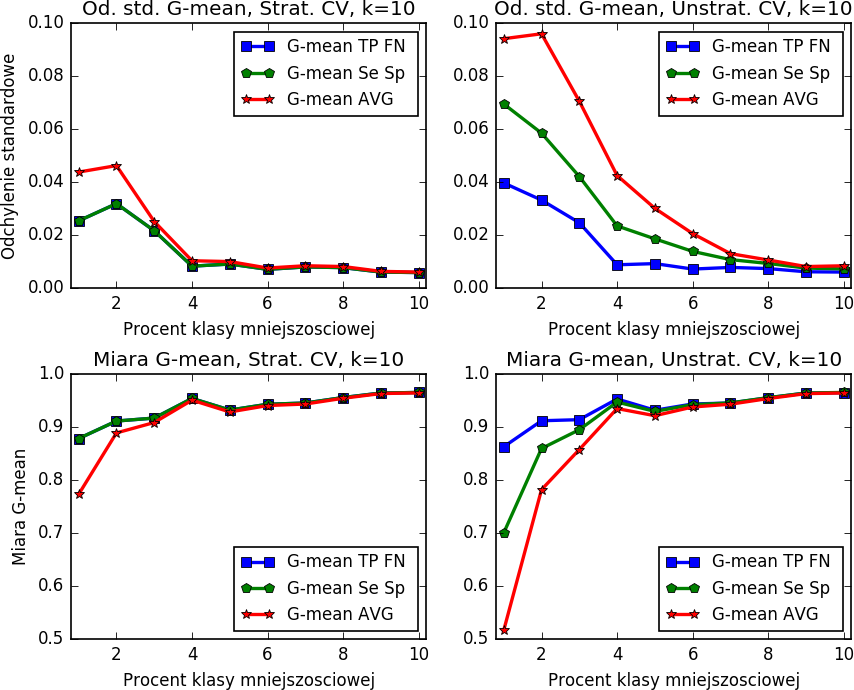
\includegraphics[width=\textwidth]{./images/miara-G-mean.png}
	\caption{Wykres odchylenia standardowego miar G-mean oraz średniej miar G-mean w zależności od wielkości klasy mniejszościowej dla równomiernego oraz losowego sprawdzianu krzyżowego (k=10).}
	\label{fig:wykresgmean}
\end{figure}
\subsubsection{Krzywa ROC i miara AUC}
Wartość AUC w sprawdzianie krzyżowym można skonstruować na dwa sposoby. W pierwszej metodzie, konstruuje się krzywą ROC oraz oblicza się AUC dla każdego k klasyfikatora. Następnie oblicza się $AUC_{AVG}$ poprzez obliczenie średniej:
\[AUC_{AVG} := \frac{1}{k} \sum_{i=1}^{k} AUC^{(i)} \]
W przypadku sprawdzianu krzyżowego z losowym rozkładem klas, może okazać się, że nie sklasyfikowano żadnego przykładu pozytywnego. Wtedy skonstruowanie krzywej ROC oraz obliczenie AUC będzie niemożliwe. W takich przypadkach podczas obliczania $AUC_{AVG}$ można pominąć taki wynik. \par
Drugim sposobem jest połączenie prawdopodobieństwa przykładów testowych z każdej iteracji. Z połączonych obserwacji, konstruuje się jedną krzywą ROC i oblicza $AUC_{merge}$. Korzystając z tego sposobu, zakłada się, że klasyfikator ma dobrze skalibrowane określanie prawdopodobieństwa.  Test obu metod zostały przeprowadzone z użyciem skryptu $test_roc.py$ i danych $tranfusion$. Wygenerowane krzywe (wykres \ref{fig:cv_roc}) ROC k klasyfikatorów różnią się od siebie kształtem oraz powierzchnią AUC. W obu sprawdzianach krzyżowych obliczona średnia $ROC_{AVG}$ oraz $AUC_{AVG}$ znajdują się pomiędzy wartościami otrzymanymi z klasyfikatorów cząstkowych (fold). Natomiast w sprawdzianie krzyżowym równomiernym wykres $ROC_{merge}$ przez większość przebiegu znajduje się poniżej części składowych, a obliczona wartość $AUC_{merge}$ jest niższa od AUC każdego klasyfikatora.
\begin{figure}[H]
	\centering
	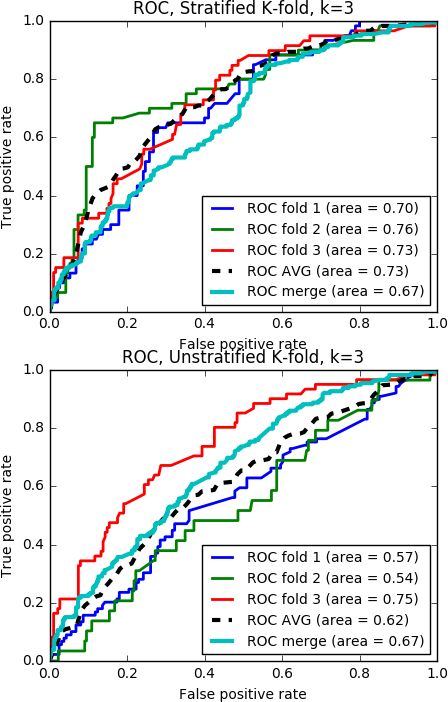
\includegraphics{./images/CV_ROC.png}
	\caption{Wykresy krzywych ROC dla klasyfikatorów ze sprawdzianu krzyżowego równomiernego i normalnego wraz z obliczoną średnią $ROC_{AVG}$ oraz $ROC_{merge}$.}
	\label{fig:cv_roc}
\end{figure}

\subsubsection{Podsumowanie}
Analizując przeprowadzone testy, najlepsze wyniki osiągnęły miary obliczone metodami opartymi na zsumowanej macierzy pomyłek oraz na łączeniu wyników testów z każdej iteracji sprawdzianu krzyżowego. Obliczone w ten sposób współczynniki miały najbardziej stabilne wyniki, najmniejszy błąd oraz wariancję. Poniżej przedstawiono tabelę (\ref{przykladoblwsp}) z obliczonymi współczynnikami na różne sposoby. Mimo równomiernego rozkładu klas, klasyfikator w części numer 2 nie rozpoznał ani jednego przykładu pozytywnego. W efekcie czułość oraz precyzja musiały zostać ustawione na 0, skutkiem czego miara G-mean oraz F1 dla tej części wynoszą 0. Pochodną tego zdarzenia jest zaniżenie wszystkich wartości średnich miar (oznaczonych w tabeli jako AVG). W dalszej części pracy, wszystkie miary w sprawdzianie krzyżowym, będą obliczane nad podstawie wspólnej macierzy pomyłek. 
\begin{table}[H]
	\begin{center}
		\resizebox{\textwidth}{!}{%
			\begin{tabular}{cccccccccccc}%
				\textbf{k-fold} & \textbf{Pos} & \textbf{Neg} & \textbf{TP} & \textbf{FP} & \textbf{FN} & \textbf{TN} & \textbf{Se} & \textbf{Sp} & \textbf{Pre} & \textbf{G-Mean} & $\mathbf{F_{1}}$\\
				\hline
				1 & 3 & 97 & 2 & 0 & 1 & 97 &  0,67 & 1,00 & 1,00 & 0,82 & 0,80\\
				2 & 3 & 97 & 0 & 0 & 3 & 97 &  0,00 & 1,00 & 0,00 & 0,00 & 0,00\\
				3 & 3 & 97 & 3 & 4 & 1 & 93 &  0,75 & 0,96 & 0,43 & 0,85 & 0,55\\

				  &   &    &   &   &   & \textbf{AVG}      & \textbf{0,47} & \textbf{0,99} & \textbf{0,48} & \textbf{0,55} & \textbf{0,45} \\
				  &   &    &   &   &   & \textbf{tp,fp,tn} & \textbf{0,50} & \textbf{0,99} & \textbf{0,56} & \textbf{0,70} & \textbf{0,53} \\
				  &   &    &   &   &   &  &  &  &  \multicolumn{3}{ c }{$\mathbf{G_{Se, Sp} =0,68}$ $\mathbf{F_{Pre, Re} =0,47}$}  \\
				

			\end{tabular}}%
			\caption{Przykład obliczonych miar dla równomiernego sprawdzianu krzyżowego. Dla k=2, gdzie nie było pozytywnie sklasyfikowanych przykładów, wartości sensitivity, precision, $F_1$ zostały ustawione na 0, aby uniknąć dzielenia przez zero. W wierszu oznaczonym jako "tp,fp,tn", wskaźniki zostały obliczone na podstawie wspólnej macierzy pomyłek.}
			\label{przykladoblwsp}
	\end{center}
\end{table}



\todo{dac odnosnik do rozdzialu}
\section{Balansowanie niezrównoważonych zbiorów z sprawdzianem krzyżowym}
Balansowanie niezrównoważonych zbiorów danych wykonuje się w celu poprawy klasyfikacji klasy mniejszościowej. Istnieją różne techniki balansowania zbiorów(opisanych w rozdziale ), są to między innymi: usuwanie przykładów z klasy większościowej oraz dodawanie nowych obserwacji z klasy mniejszościowej. Oceniając klasyfikator z wykorzystaniem sprawdzianu krzyżowego, bilansowanie zbiorów można wykonać przed sprawdzianem krzyżowym oraz w trakcie trwania sprawdzianu, każdorazowo po stworzeniu zbioru uczącego. W przypadku generowania nowych obserwacji (oversampling), metoda pierwsza może prowadzić do nadmiernego dopasowania. Sprawdzian krzyżowy k-krotny, dzieli główny zbiór danych na $k$ części i buduje klasyfikator w oparciu $k-1$ części. Następnie testuje go w oparciu o część nr. $k$. Może wystąpić taka sytuacja, że ocena klasyfikatora będzie odbywała się w oparciu o sztuczne przykłady, które były wygenerowane na podstawie danych tworzących zbiór uczący. Taka sytuacja wypacza cel wykonywania sprawdzianu krzyżowego, który polega na wykonywaniu uczenia i testowania na różnych danych. Wykonanie bilansowania przed sprawdzianem krzyżowym może prowadzić do nadmiernego dopasowania klasyfikatora oraz do zawyżenia oceny. Celem testu było sprawdzenie, z wykorzystaniem, której metody można otrzymać bardziej wiarygodne wyniki. Aby sprawdzić obie metody, każdy początkowy zbiór danych został podzielony na zbiór testowy (zawierający 80\% wszystkich przykładów) oraz na zbiór walidacyjny (20\%). Wykonano zbilansowany podział danych, tj. każdy zbiór zawierał proporcjonalnie takie same ilości obu klas. Zbiór walidacyjny został wydzielony w celu poddania dodatkowej ocenie każdego $k$ klasyfikatora. Mając dodatkowy zbiór z danymi nieznanymi model, można sprawdzić w jakim stopniu poprawnie generalizuje dane uczące oraz porównać otrzymane wyniki z wynikami sprawdzianu krzyżowego. Dla pierwszego sposobu, w kolejnym etapie, wygenerowano nowe sztuczne próbki klasy mniejszościowej z wykorzystaniem metody oversampling SMOTE, a następnie poddano ocenie klasyfikator z wykorzystaniem sprawdzianu krzyżowego oraz dodatkowego zbioru walidacyjnego w każdej iteracji. Natomiast w drugim sposobie, dodatkowe sztuczne próbki generowane były dopiero w momencie utworzenia $k$ zbioru uczącego. Dodatkowa walidacja odbywała się tak samo jak w pierwszym sposobie. Badanie wykonano na prawdziwych danych (opisanych w tej pracy), z wykorzystaniem klasyfikatorów: drzewo decyzyjne, kNN, naiwny klasyfikator Bayesa oraz SVM. Przedstawiony niżej test znajduje się w pliku $cross\_val\_oversampling.py$. Ze względu na dużą objętość wyników, w pracy przedstawiono tylko dane dla drzewa decyzyjnego. \par
Analizując otrzymane wyniki (tabela \ref{CVoversampling1} i \ref{CVoversampling2}) zauważono bardzo dobre wyniki klasyfikatora dla danych poddanych oversamplingowi przed sprawdzianem krzyżowym. Niestety, badając klasyfikator nieznanym dla niego zbiorem walidacyjnym otrzymane rezultaty były zdecydowanie gorsze. Porównując otrzymane wyniki z sprawdzianu krzyżowego oraz z nieznanego klasyfikatorowi zbioru walidacyjnyjego, spostrzeżono znaczne zawyżanie wyników (dla miary G-mean, wyniki jest średnio wyższy o 0.20 oraz tak samo w stosunku do miary G-mean z metody drugiej). Świadczy to o nadmiernym dopasowaniu klasyfikatora do danych i o zawyżaniu wyników jakości klasyfikacji przez tą metodę. W drugiej metodzie, wyniki pomiarów pomiędzy sprawdzianem krzyżowym oraz zbiorem walidacyjnym nie różnią się tak bardzo. Dla miary G-mean w większości baz, otrzymany wyniki z sprawdzianu krzyżowego jest nieznacznie niższy od wyniku z zbioru walidacyjnego. \par
Wnioskiem wynikającym z powyższego badania jest konieczność stosowania oversamplingu danych w trakcie sprawdzianu krzyżowego, tak aby zbiór testowy nie zawierał sztucznie wygenerowanych próbek. Ocena klasyfikacji tą metodą, daje najbardziej wiarygodne wyniki.
\begin{table}[H]
	\begin{center}
		\resizebox{\textwidth}{!}{%
			\begin{tabular}{|c|c|c|c|c|c|c|c|c|c|}%
				\hline%
				&\multicolumn{4}{|c|}{Decision Tree}&\multicolumn{4}{|c|}{Decision Tree TEST}&\\%
				\cline{2%
					-%
					10}%
				& Sp & F1 & G & AUC & Sp &F1 & $G_t$&AUC& $G - G_t$\\%
				\hline%
				abalone0\_4&0.99&0.99&0.99&0.99&0.79&0.58&0.88&0.88&0.11\\%
				abalone041629&0.92&0.91&0.9&0.9&0.5&0.34&0.66&0.69&0.24\\%
				abalone16\_29&0.93&0.92&0.92&0.92&0.51&0.34&0.68&0.71&0.24\\%
				balance\_scale&0.92&0.9&0.9&0.9&0.04&0.04&0.19&0.47&0.71\\%
				breast\_cancer&0.74&0.74&0.74&0.75&0.47&0.45&0.59&0.61&0.15\\%
				bupa&0.69&0.66&0.65&0.65&0.57&0.55&0.6&0.6&0.05\\%
				car&1.0&1.0&1.0&1.0&0.9&0.95&0.95&0.95&0.05\\%
				cmc&0.8&0.81&0.81&0.81&0.39&0.37&0.55&0.6&0.26\\%
				ecoli&0.93&0.93&0.92&0.93&0.81&0.62&0.86&0.86&0.06\\%
				german&0.74&0.75&0.75&0.75&0.44&0.44&0.58&0.59&0.17\\%
				glass&0.96&0.93&0.93&0.93&0.56&0.5&0.73&0.75&0.2\\%
				haberman&0.72&0.73&0.74&0.74&0.35&0.35&0.52&0.56&0.22\\%
				heart\_cleveland&0.88&0.87&0.86&0.86&0.24&0.29&0.47&0.59&0.39\\%
				hepatitis&0.92&0.86&0.84&0.85&0.39&0.33&0.54&0.57&0.3\\%
				horse\_colic&0.84&0.82&0.82&0.82&0.65&0.66&0.73&0.73&0.09\\%
				ionosphere&0.88&0.88&0.88&0.88&0.87&0.81&0.86&0.86&0.02\\%
				new\_thyroid&0.96&0.96&0.96&0.96&1.0&0.95&0.99&0.99&{-}0.03\\%
				postoperative&0.68&0.7&0.71&0.71&0.33&0.34&0.51&0.56&0.2\\%
				seeds&0.97&0.96&0.96&0.96&0.62&0.7&0.76&0.77&0.2\\%
				solar\_flare&0.96&0.96&0.96&0.97&0.13&0.19&0.36&0.63&0.6\\%
				transfusion&0.76&0.75&0.75&0.77&0.4&0.35&0.54&0.58&0.21\\%
				vehicle&0.89&0.92&0.92&0.92&0.72&0.76&0.83&0.83&0.09\\%
				vertebal&0.89&0.86&0.85&0.85&0.73&0.66&0.75&0.75&0.1\\%
				yeastME1&0.99&0.99&0.99&0.99&0.72&0.68&0.84&0.85&0.15\\%
				yeastME2&0.98&0.96&0.96&0.96&0.69&0.42&0.81&0.82&0.15\\%
				yeastME3&0.96&0.96&0.96&0.96&0.66&0.65&0.79&0.81&0.17\\%
				\hline%
			\end{tabular}}%
			\caption{Wyniki sprawdzianu krzyżowego (metoda pierwsza) drzewa decyzyjnego z oversampling SMOTE. Dane w kolumnach "Decision Tree TEST" to wyniki otrzymane na podstawie zbioru walidacyjnego. Ostatnia kolumna zawiera różnicę  miar G ze sprawdzianu krzyżowego i zbioru walidacyjnego $G-G_T$ (im bliżej zera tym lepiej).}
			\label{CVoversampling1}
		\end{center}
\end{table}


\begin{table}[H]
	\begin{center}
		\resizebox{\textwidth}{!}{%
		\begin{tabular}{|c|c|c|c|c|c|c|c|c|c|}%
			\hline%
			&\multicolumn{4}{|c|}{Decision Tree}&\multicolumn{4}{|c|}{Decision Tree TEST}&\\%
			\cline{2%
				-%
				10}%
				& Sp & F1 & G & AUC & Sp &F1 & $G_t$&AUC& $G - G_t$\\%
			\hline%
			abalone0\_4&0.68&0.54&0.82&0.83&0.77&0.58&0.87&0.88&{-}0.05\\%
			abalone041629&0.42&0.31&0.61&0.65&0.45&0.32&0.63&0.67&{-}0.02\\%
			abalone16\_29&0.39&0.27&0.59&0.64&0.52&0.34&0.68&0.71&{-}0.09\\%
			balance\_scale&0.03&0.02&0.15&0.47&0.04&0.03&0.19&0.46&{-}0.04\\%
			breast\_cancer&0.41&0.4&0.55&0.57&0.41&0.4&0.55&0.57&0.0\\%
			bupa&0.54&0.54&0.6&0.6&0.55&0.56&0.62&0.62&{-}0.02\\%
			car&0.98&0.98&0.99&0.99&0.91&0.95&0.95&0.95&0.04\\%
			cmc&0.38&0.36&0.55&0.59&0.39&0.37&0.56&0.61&{-}0.01\\%
			ecoli&0.54&0.53&0.71&0.74&0.62&0.58&0.76&0.78&{-}0.05\\%
			german&0.55&0.54&0.66&0.67&0.5&0.49&0.62&0.63&0.04\\%
			glass&0.14&0.16&0.37&0.54&0.56&0.56&0.73&0.76&{-}0.36\\%
			haberman&0.49&0.42&0.58&0.59&0.4&0.36&0.53&0.55&0.05\\%
			heart\_cleveland&0.43&0.35&0.61&0.65&0.24&0.29&0.48&0.59&0.13\\%
			hepatitis&0.5&0.52&0.67&0.69&0.72&0.58&0.77&0.77&{-}0.1\\%
			horse\_colic&0.78&0.77&0.82&0.82&0.65&0.66&0.73&0.73&0.09\\%
			ionosphere&0.82&0.81&0.85&0.85&0.85&0.81&0.85&0.85&0.0\\%
			new\_thyroid&0.88&0.86&0.92&0.92&0.94&0.87&0.95&0.95&{-}0.03\\%
			postoperative&0.32&0.27&0.44&0.48&0.33&0.3&0.47&0.48&{-}0.03\\%
			seeds&0.95&0.91&0.94&0.94&0.62&0.68&0.75&0.76&0.19\\%
			solar\_flare&0.21&0.2&0.45&0.62&0.13&0.18&0.36&0.63&0.09\\%
			transfusion&0.36&0.34&0.52&0.58&0.39&0.35&0.54&0.57&{-}0.02\\%
			vehicle&0.82&0.82&0.88&0.88&0.76&0.79&0.85&0.85&0.03\\%
			vertebal&0.66&0.68&0.75&0.76&0.63&0.63&0.72&0.73&0.03\\%
			yeastME1&0.63&0.59&0.79&0.81&0.72&0.69&0.84&0.86&{-}0.05\\%
			yeastME2&0.29&0.2&0.53&0.62&0.41&0.3&0.63&0.68&{-}0.1\\%
			yeastME3&0.81&0.77&0.88&0.89&0.68&0.68&0.81&0.82&0.07\\%
			\hline%
		\end{tabular}}%
			\caption{Wyniki sprawdzianu krzyżowego (metoda druga) drzewa decyzyjnego z oversampling SMOTE. Dane w kolumnach "Decision Tree TEST" to wyniki otrzymane na podstawie zbioru walidacyjnego. Ostatnia kolumna zawiera różnicę  miar G ze sprawdzianu krzyżowego i zbioru walidacyjnego $G-G_T$ (im bliżej zera tym lepiej).}
			\label{CVoversampling2}
	\end{center}
\end{table}

\section{Porównanie klasyfikatorów}
\todo{przetestsowa wszystkie klasyfkatory, z metodami pre i bez}

Porównanie klasyfikatorów z domyślnymi ustawieniami, na takich samych typach danych. Jeżeli w tabelce występuje 0, to klasyfikator całkowicie błędnie klasyfikuje klasę mniejszościową.

			\begin{table}[H]
				\begin{center}
					\resizebox{\textwidth}{!}{%
						\begin{tabular}{c|cccccccccc}%
							\hline%
							&Tree&BG&(3)&B(3)&(5)&B(5)&(10)&B(10)&(20)&B(20)\\%
							\hline%
							abalone0\_4&0.71&0.74&\textbf{0.82}&0.78&0.74&0.73&0.71&0.74&0.69&0.74\\%
							\hline%
							abalone041629&\textbf{0.58}&0.53&0.39&0.36&0.48&0.48&0.56&0.53&\textbf{0.58}&0.53\\%
							\hline%
							abalone16\_29&0.51&0.46&0.16&0.0&0.44&0.4&\textbf{0.52}&0.46&0.51&0.46\\%
							\hline%
							balance\_scale&\textbf{0.27}&0.0&0.0&0.0&0.2&0.0&\textbf{0.27}&0.0&\textbf{0.27}&0.0\\%
							\hline%
							breast\_cancer&0.54&0.58&0.51&0.52&0.51&0.54&0.54&\textbf{0.59}&0.55&0.58\\%
							\hline%
							car&\textbf{0.96}&\textbf{0.96}&0.0&0.0&0.95&0.95&\textbf{0.96}&\textbf{0.96}&\textbf{0.96}&\textbf{0.96}\\%
							\hline%
							cmc&0.52&0.48&0.22&0.15&\textbf{0.54}&0.48&0.5&0.5&0.51&0.49\\%
							\hline%
							ecoli&0.71&0.72&0.63&0.65&\textbf{0.75}&0.72&0.71&0.72&0.71&0.72\\%
							\hline%
							glass&\textbf{0.52}&0.0&0.24&0.0&\textbf{0.52}&0.0&\textbf{0.52}&0.0&\textbf{0.52}&0.0\\%
							\hline%
							haberman&0.47&0.48&\textbf{0.58}&0.51&0.49&0.49&0.48&0.49&0.47&0.48\\%
							\hline%
							heart\_cleveland&\textbf{0.48}&0.23&0.17&0.0&0.42&0.23&\textbf{0.48}&0.23&\textbf{0.48}&0.23\\%
							\hline%
							hepatitis&\textbf{0.69}&\textbf{0.69}&0.6&0.56&\textbf{0.69}&0.67&\textbf{0.69}&\textbf{0.69}&\textbf{0.69}&\textbf{0.69}\\%
							\hline%
							new\_thyroid&\textbf{0.94}&\textbf{0.94}&0.9&0.92&\textbf{0.94}&\textbf{0.94}&\textbf{0.94}&\textbf{0.94}&\textbf{0.94}&\textbf{0.94}\\%
							\hline%
							postoperative&\textbf{0.36}&0.26&0.0&0.0&0.19&0.27&\textbf{0.36}&0.26&\textbf{0.36}&0.26\\%
							\hline%
							solar\_flare&\textbf{0.37}&0.34&0.0&0.0&\textbf{0.37}&0.26&\textbf{0.37}&0.34&\textbf{0.37}&0.34\\%
							\hline%
							transfusion&0.43&0.46&0.38&0.28&0.45&\textbf{0.47}&0.43&0.46&0.43&0.46\\%
							\hline%
							vehicle&0.89&0.94&0.71&0.71&0.89&\textbf{0.95}&0.9&0.94&0.89&0.94\\%
							\hline%
							yeastME1&0.85&0.81&\textbf{0.86}&0.72&0.81&0.79&0.85&0.81&0.85&0.81\\%
							\hline%
							yeastME2&\textbf{0.66}&0.5&0.24&0.14&0.65&0.5&\textbf{0.66}&0.5&\textbf{0.66}&0.5\\%
							\hline%
							yeastME3&0.81&0.84&\textbf{0.88}&0.87&0.84&0.85&0.81&0.84&0.81&0.84\\%
							\hline%
							bupa&0.64&\textbf{0.67}&0.6&0.6&\textbf{0.67}&0.66&0.65&\textbf{0.67}&0.65&\textbf{0.67}\\%
							\hline%
							german&0.63&0.64&0.45&0.47&0.63&0.64&0.62&\textbf{0.65}&0.62&0.64\\%
							\hline%
						\end{tabular}
}%
						\caption{F1}
						\label{tab4}
					\end{center}
				\end{table}			\begin{table}[H]
				\begin{center}
					\resizebox{\textwidth}{!}{%
						\begin{tabular}{c|cccccccccc}%
							\hline%
							&Tree&BG&(3)&B(3)&(5)&B(5)&(10)&B(10)&(20)&B(20)\\%
							\hline%
							abalone0\_4&0.71&0.74&\textbf{0.82}&0.78&0.74&0.73&0.71&0.74&0.69&0.74\\%
							\hline%
							abalone041629&\textbf{0.58}&0.53&0.39&0.36&0.48&0.48&0.56&0.53&\textbf{0.58}&0.53\\%
							\hline%
							abalone16\_29&0.51&0.46&0.16&0.0&0.44&0.4&\textbf{0.52}&0.46&0.51&0.46\\%
							\hline%
							balance\_scale&\textbf{0.27}&0.0&0.0&0.0&0.2&0.0&\textbf{0.27}&0.0&\textbf{0.27}&0.0\\%
							\hline%
							breast\_cancer&0.54&0.58&0.51&0.52&0.51&0.54&0.54&\textbf{0.59}&0.55&0.58\\%
							\hline%
							car&\textbf{0.96}&\textbf{0.96}&0.0&0.0&0.95&0.95&\textbf{0.96}&\textbf{0.96}&\textbf{0.96}&\textbf{0.96}\\%
							\hline%
							cmc&0.52&0.48&0.22&0.15&\textbf{0.54}&0.48&0.5&0.5&0.51&0.49\\%
							\hline%
							ecoli&0.71&0.72&0.63&0.65&\textbf{0.75}&0.72&0.71&0.72&0.71&0.72\\%
							\hline%
							glass&\textbf{0.52}&0.0&0.24&0.0&\textbf{0.52}&0.0&\textbf{0.52}&0.0&\textbf{0.52}&0.0\\%
							\hline%
							haberman&0.47&0.48&\textbf{0.58}&0.51&0.49&0.49&0.48&0.49&0.47&0.48\\%
							\hline%
							heart\_cleveland&\textbf{0.48}&0.23&0.17&0.0&0.42&0.23&\textbf{0.48}&0.23&\textbf{0.48}&0.23\\%
							\hline%
							hepatitis&\textbf{0.69}&\textbf{0.69}&0.6&0.56&\textbf{0.69}&0.67&\textbf{0.69}&\textbf{0.69}&\textbf{0.69}&\textbf{0.69}\\%
							\hline%
							new\_thyroid&\textbf{0.94}&\textbf{0.94}&0.9&0.92&\textbf{0.94}&\textbf{0.94}&\textbf{0.94}&\textbf{0.94}&\textbf{0.94}&\textbf{0.94}\\%
							\hline%
							postoperative&\textbf{0.36}&0.26&0.0&0.0&0.19&0.27&\textbf{0.36}&0.26&\textbf{0.36}&0.26\\%
							\hline%
							solar\_flare&\textbf{0.37}&0.34&0.0&0.0&\textbf{0.37}&0.26&\textbf{0.37}&0.34&\textbf{0.37}&0.34\\%
							\hline%
							transfusion&0.43&0.46&0.38&0.28&0.45&\textbf{0.47}&0.43&0.46&0.43&0.46\\%
							\hline%
							vehicle&0.89&0.94&0.71&0.71&0.89&\textbf{0.95}&0.9&0.94&0.89&0.94\\%
							\hline%
							yeastME1&0.85&0.81&\textbf{0.86}&0.72&0.81&0.79&0.85&0.81&0.85&0.81\\%
							\hline%
							yeastME2&\textbf{0.66}&0.5&0.24&0.14&0.65&0.5&\textbf{0.66}&0.5&\textbf{0.66}&0.5\\%
							\hline%
							yeastME3&0.81&0.84&\textbf{0.88}&0.87&0.84&0.85&0.81&0.84&0.81&0.84\\%
							\hline%
							bupa&0.64&\textbf{0.67}&0.6&0.6&\textbf{0.67}&0.66&0.65&\textbf{0.67}&0.65&\textbf{0.67}\\%
							\hline%
							german&0.63&0.64&0.45&0.47&0.63&0.64&0.62&\textbf{0.65}&0.62&0.64\\%
							\hline%
						\end{tabular}
					}%
					\caption{F1}
					\label{tab4}
				\end{center}
			\end{table}